\documentclass[12pt,letterpaper]{article}

\usepackage{tabularx}
\usepackage{svg}
\usepackage{tikz}
\usepackage{pdflscape}
\usepackage{siunitx}
\usepackage{caption}
\usepackage{subcaption}
\usepackage{float}
\usepackage[numbers]{natbib}
\usepackage{setspace}
\usepackage[left=1.5in,right=1in,top=1in,bottom=1in]{geometry}
\usepackage[scaled]{helvet}
\usepackage[export]{adjustbox}
\renewcommand\familydefault{\sfdefault}
\usepackage{etoolbox}
\apptocmd{\thebibliography}{\raggedright}{}{}
\usepackage[hidelinks]{hyperref}
\hypersetup{ colorlinks, citecolor=black,
  filecolor=black,
  linkcolor=black,
  urlcolor=blue,
  pdftitle={Insulin Temperature Warning System: Final Report},
  pdfpagemode=FullScreen,
}
\usepackage{bookmark}
\bookmarksetup{
  numbered,
  open,
}

\newcommand\createfigurewsvg[3]{
 \begin{figure}[H]
  \begin{center}
    \centering\includesvg[width=0.9\textwidth]{#1}
    \caption{#2}
    \label{#3}
  \end{center}
 \end{figure}
}

\newcommand\createfigurew[3]{
  \begin{center}
  \begin{figure}[H]
    \centering \includegraphics[width=\textwidth]{#1}
    \caption{#2}
    \label{#3}
  \end{figure}
  \end{center}
}

\newcommand\createfigurel[3]{
  \begin{center}
  \begin{figure}[H]
    \centering \includegraphics[height=0.8\textheight]{#1}
    \caption{#2}
    \label{#3}
  \end{figure}
  \end{center}
}

\begin{document}
\linespread{1.0}
\begin{titlepage}
  \begin{center}
    \large{University of Puerto Rico\\
    Mayagüez Campus\\
    \vspace{\baselineskip}
    Department of Electrical and Computer Engineering\\}
    \vspace{6cm}
    \Huge{\underline{Insulin Temperature Warning System}\\}
    \vspace{0.5\baselineskip}
    \large by\\
    Fabio J. Matos Nieves\\
    Enrique Chompré\\
    Guillermo Colón\\
    Rubén Marrero\\
    \vspace{3.5cm}
    For: Professor Manuel Jimenez\\
    Course: INEL 4217 Seccion 096\\
    Date: Febuary 2, 2023\\
    \normalsize

  \end{center}
\end{titlepage}

\linespread{2.0}
\section*{Abstract}
The purpose of this document is outlining a design for a pair of devices that monitor the temperature of insulin, making sure that it meets the safe storage guidelines in a mass storage context. This document contains the system conception, system architecture \& functionality, specifications and market description as well as the project time table, design criteria and the opinion of the client of this design.

\newpage
\tableofcontents
\listoffigures
\listoftables
\section{Introduction}
In 2017 hurricane Maria devastated the northeastern Caribbean, particularly Dominica, Saint Croix, and Puerto Rico. In the wake of the storm, Puerto Rico suffered the longest blackout in US history and the second longest blackout in recorded human history\cite{WorldSecondLargest}. The revised death count attributable to the hurricane was 2,975 people\cite{HurricaneMariaCaused2018}. According to an investigation by the New York Times, deaths caused by  sepsis, pneumonia, emphysema, diabetes, and Alzheimer's and Parkinson's spiked in the two months following the hurricane\cite{roblesOfficialTollPuerto2017}. The whole island of Puerto Rico was declared a disaster zone by the Federal Emergency Management Agency (FEMA) and it wasn't until four to eight months after the storm that most of the population had electricity and running water after the storm. The Puerto Rican electrical grid also collapsed in the aftermath of hurricane Fiona in September of 2022. Puerto Rico also has a sizable portion of the adult population with diabetes and a large portion of those diagnosed with diabetes require insulin to survive\cite{DiabetesPrevalencePopulation}. The rationale for this project is to provide a tool for users of insulin to be sure that their medication is safe and effective in normal and post-disaster conditions. The problem is that there has not been a way to monitor the storage conditions of insulin in a consumer setting in normal/post-disaster conditions. This project's solution to this problem is to create a micro-controller based design that can:
\begin{itemize}
  \item Monitor the temperature of the insulin.
  \item Check if a power-outage has occurred.
  \item Warn the main unit if the temperature has exceeded \textnormal{$15^{\circ}C$} and turn on a warning light on the sub unit.
  \item Record the temperature, time-stamp and power-availability on a log file on the main unit.
  \item Let the main unit warn an operator if a sub-unit has exceeded temperature guidelines.
  \item The main unit send its logging information to a device.
\end{itemize}

\section{Theoretical Background}
The major considerations for laying out the requirements for this design were the state guidelines for insulin storage and the expiration dates for various manufacturers of insulin. According to the Centers for Disease Control (CDC)\cite{ManagingInsulinEmergency2022}, the Food and Drug Administration (FDA) \cite{researchInformationRegardingInsulin2018} and the National Institute of Health (NIH) \cite{bahendekaEADSGGuidelinesInsulin2019} along with our client, for long term storage vials of insulin ought to be stored between 2\si{\celsius} and 8\si{\celsius} and can have a shelf life of up to 2 years. With these criteria in mind, our team set of to create a design that was:
\begin{itemize}
  \item Inexpensive to manufacture
  \item Uses off the shelf parts
  \item Can operate in cold and hot environments
  \item Can be reused
  \item Easy to integrate in existing production lines
  \item Has a long battery life
  \item Can operate with/without the availability of mains power
  \item Ensured compliance with federal guidelines for insulin storage
\end{itemize}
In terms of logistics, the project had a timetable of less than 4 months from pre-proposal to final prototype. In addition, since this project was being developed in the University of Puerto Rico, Mayagüez Campus, all of the parts needed to construct the prototype needed to be shipped from overseas which constricts the timetable even further.\\

\section{System Planning}
\subsection{Top-Level System View}
\subsection{System Block Diagram}
\subsection{System State Diagram}

\section{Modular Design}
\subsection{Main Unit Power Supply}
\subsubsection{Block Diagram}
\createfigurewsvg{../Modular Design/Main-Unit-PSU/Figures/main-unit-psu.svg}{Main Unit Power Supply Architectural Diagram}{fig:main-unit-psu-bd}
\subsubsection{Schematic Diagram}
\begin{landscape}
  \begin{center}
  \begin{figure}[H]
    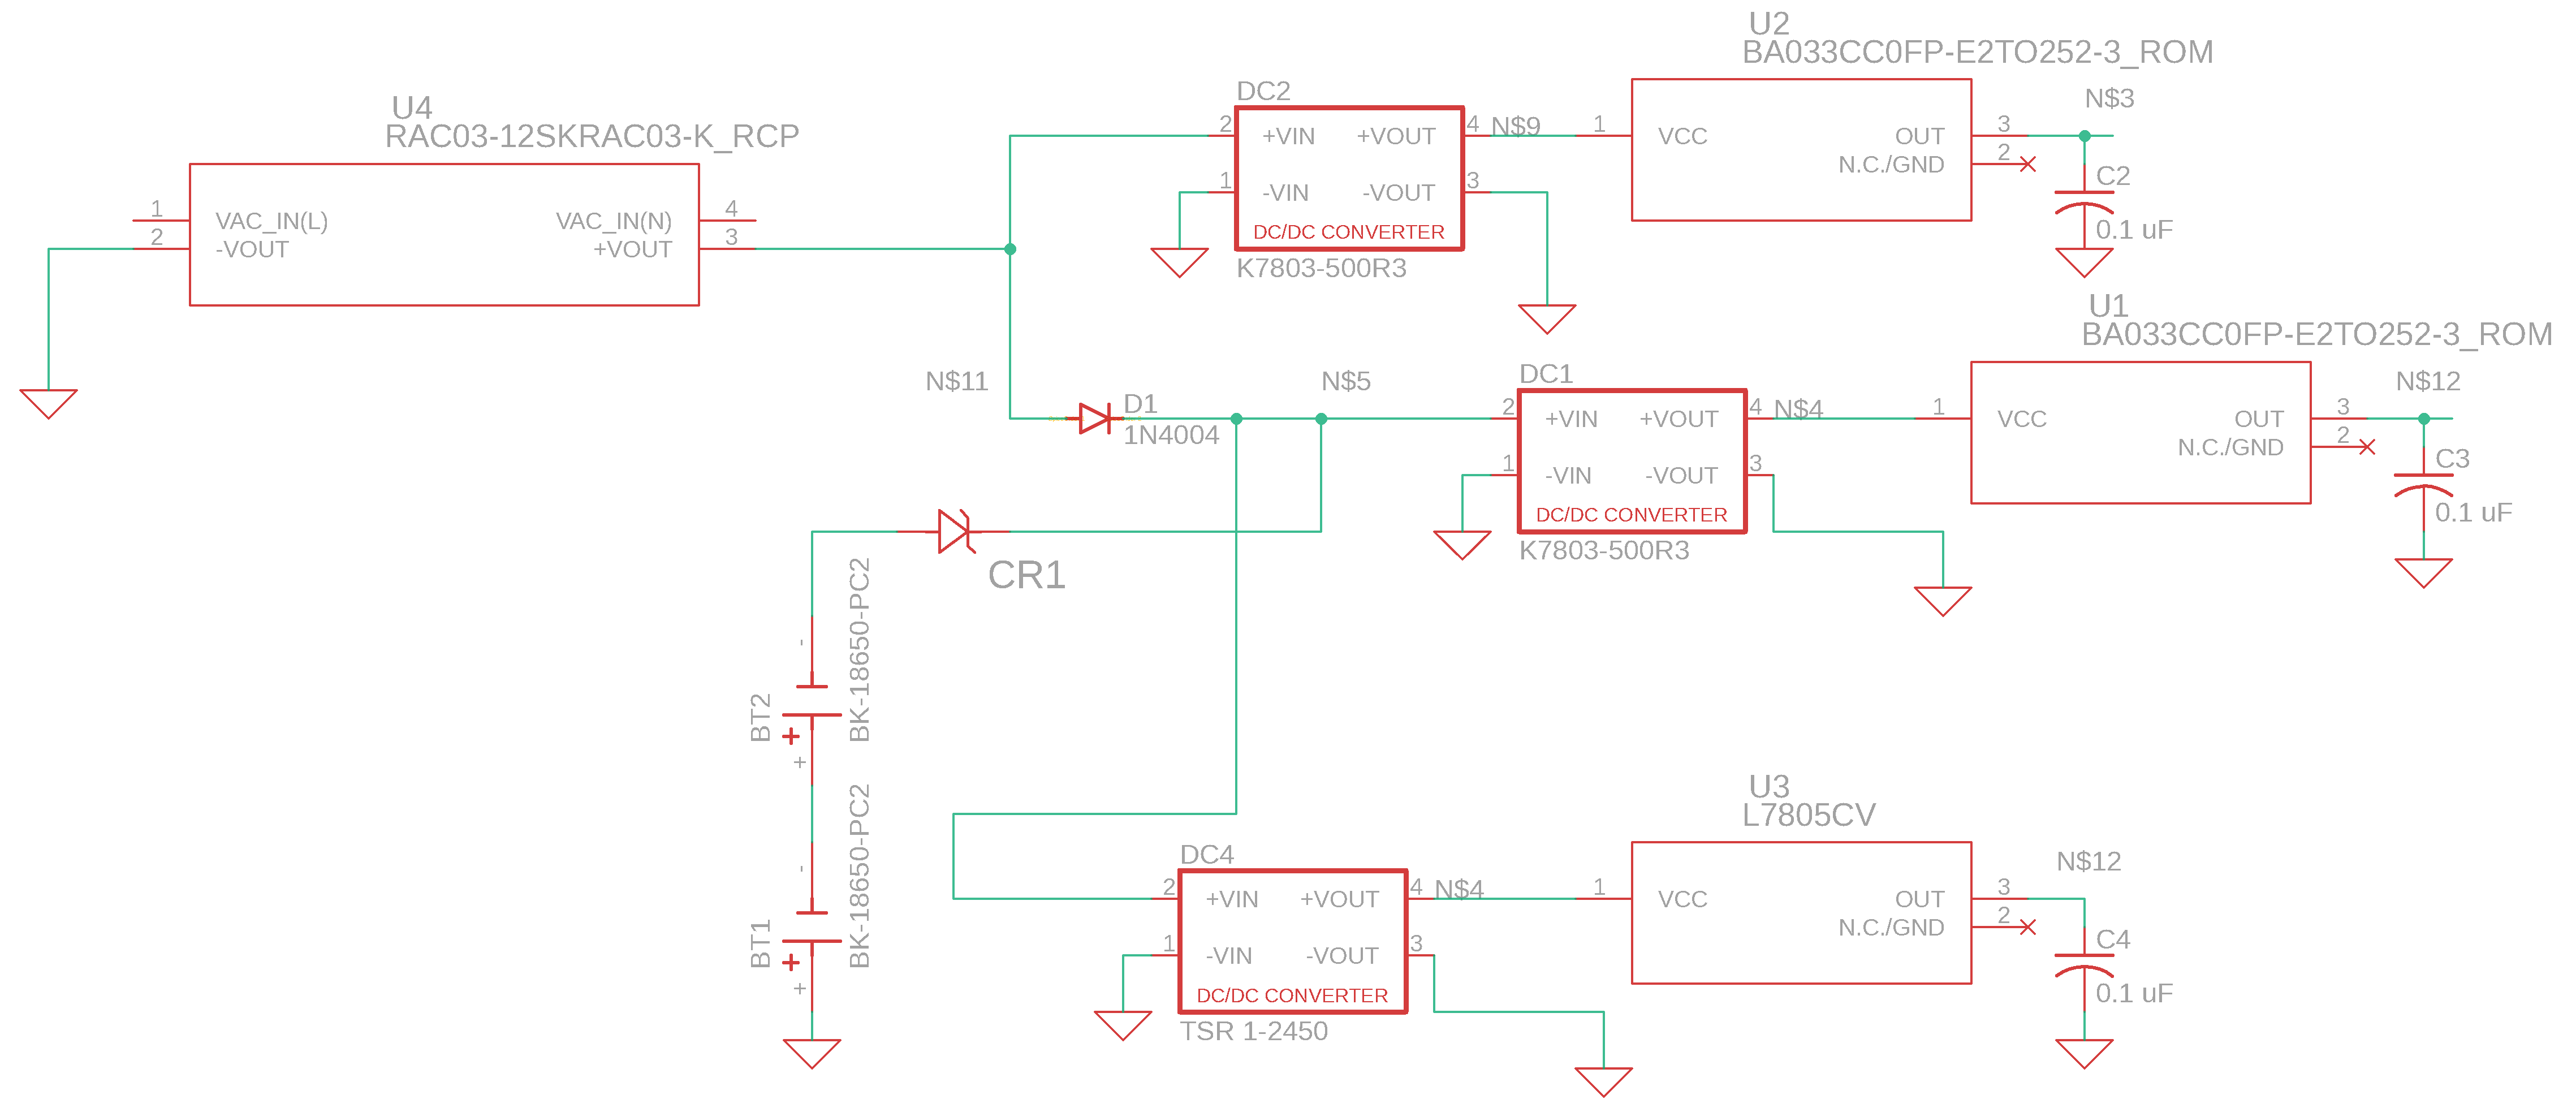
\includegraphics[width=1.6\textwidth, left]{../Modular Design/Main-Unit-PSU/Figures/main-unit-psu.png}
    \caption{Main Unit PSU Schematic}
    \label{fig:main-psu-schematic}
  \end{figure}
  \end{center}
\end{landscape}
\subsubsection{Power Analysis, Loading, Driving, and Compatibility}
According to the RAC03-12SK data sheet\cite{RAC0312SK}, the AC/DC converter can handle from 85\si{\V}AC to 264\si{\V}AC and produce 12\si{\V}DC at its output. Since this design will be tested in a 120\si{\V}AC electrical system, it is compatible.\\ At the output of the AC/DC converter, a 1N4004-G diode\cite{1N4004G} and a R78-E3.3-0.5 3.3\si{\V} DC/DC converter\cite{R78E330} (DC2) are placed in parallel. For DC2, according to its data sheet, is compatible within a voltage range of 6\si{\V} to 28\si{\V}. Since DC2 is at the output of the 12\si{\V} AC/DC converter, it is compatible.\\ At the node at the right of D1 (N\$5), when mains power is available is calculated as follows:
\begin{equation}
  V_{N\$5} = 12 -  V_{D}
  \label{eq:mains-batt-node-eqation-mains-available}
\end{equation}
where $V_{D}$ is the diode drop of the 1N4004-G which according to its data sheet is 1.1\si{\V}, resulting in $N\$5$ equal to 10.9\si{\V}. When there is mains power available, the node will be at 10.9\si{\V}, the batteries will be trying to conduct but since the voltage of the two 3.6\si{\V} cells in series will be 7.2\si{\V}, minus the diode drop of CR1\cite{1N5819} will be $7.2 - 0.55 = 6.65\si{\V}$. Therefore, the potential difference between mains power and battery power is $-4.25\si{\V}$, therefore CR1 will be placed in reverse bias and thus the batteries will not conduct, but since the negative potential difference is low, it is compatible, according to the 1N5819 data sheet\cite{1N5819}.\\ When mains power is available DC1, another K7803-500R3, will receive a voltage of 10.9\si{\V} and as mentioned above is compatible and will produce a 3.3\si{\V} output. At the outputs of both DC1,DC2 there are identical 3.3\si{\V} LDOs (BA33BC0T)\cite{BA33BC0T}, which according to their data sheet can accept up to 16\si{\V} which is compatible since U1 and U2 are being supplied by 3.3\si{\V} DC/DC converters and thus are compatible. At the outputs of U1 and U2 are C2 and C3 respectively, that are 0.1\si{\micro\farad} filtering capacitors whose voltage rating is 50\si{\V} which are compatible.\\ Going back to $N\$5$ DC4 (5\si{\V} DC/DC converter) is in parallel with DC1, thus when there is mains power available, will be supplied 10.9\si{\V}. According to the TSR 1-2450 (DC4) data sheet\cite{TSR12450} it can accept a DC voltage from 6.5\si{\V} to 36\si{\V} thus making it compatible and will output 5\si{\V} DC. At the output of DC4, a 5\si{\V} LDO is fed (L7805CV
), whose data sheet\cite{L7805CV} says that it can handle up to 36\si{\V} thus making it compatible since the output of DC4 is 5\si{\V}. Similarly to C3 and C4, a 0.1\si{\micro\farad} capacitor is placed in parallel with the output and is compatible since it has the same voltage rating of 50\si{\V}.\\ When mains power is not available DC2 will shutdown and D1 will be placed in reverse bias since CR1 will be conducting due to $N\$5$ will be at 0\si{\V} when mains power is not available and then will be placed at 6.65\si{\V}. Since DC1, DC2 and DC4 all have a minimum voltage less than 6.65\si{\V} they are all compatible and the LDOs and capacitors will operate as normal.
\subsubsection{Reliability \& Design Criteria}
The power supply for the main unit has to be working 100\% of the time since the main unit is required for the operation of the system. Because of this requirement the main power supply has an integrated battery backup switches automatically when mains power is not available and then can last for an extended period of time without the mains power available.
\subsubsection{Level of Completion}
\begin{table}[!ht]
  \begin{tabularx}{\textwidth}{|X|X|}
    \hline
    \multicolumn{2}{|X|}{Main Unit PSU}\\
    \hline
    Integration&\begin{itemize}
                  \item 4\si{\V} Power Rail
                  \item 3.3\si{\V} Power Rail
                  \item 3.3\si{\V} Power Sense
                  \item Automatic Power Source Switching
                \end{itemize}\\
    \hline
  \end{tabularx}
\end{table}

\subsection{Sub Unit Power Supply}
\subsubsection{Block Diagram}
\createfigurewsvg{../Modular Design/Sub-Unit-PSU/Figures/sub-unit-psu.svg}{Sub Unit Power Supply Architectural Diagram}{fig:sub-unit-psu-bd}
\subsubsection{Schematic Diagram}
\begin{landscape}
  \begin{center}
  \begin{figure}[H]
    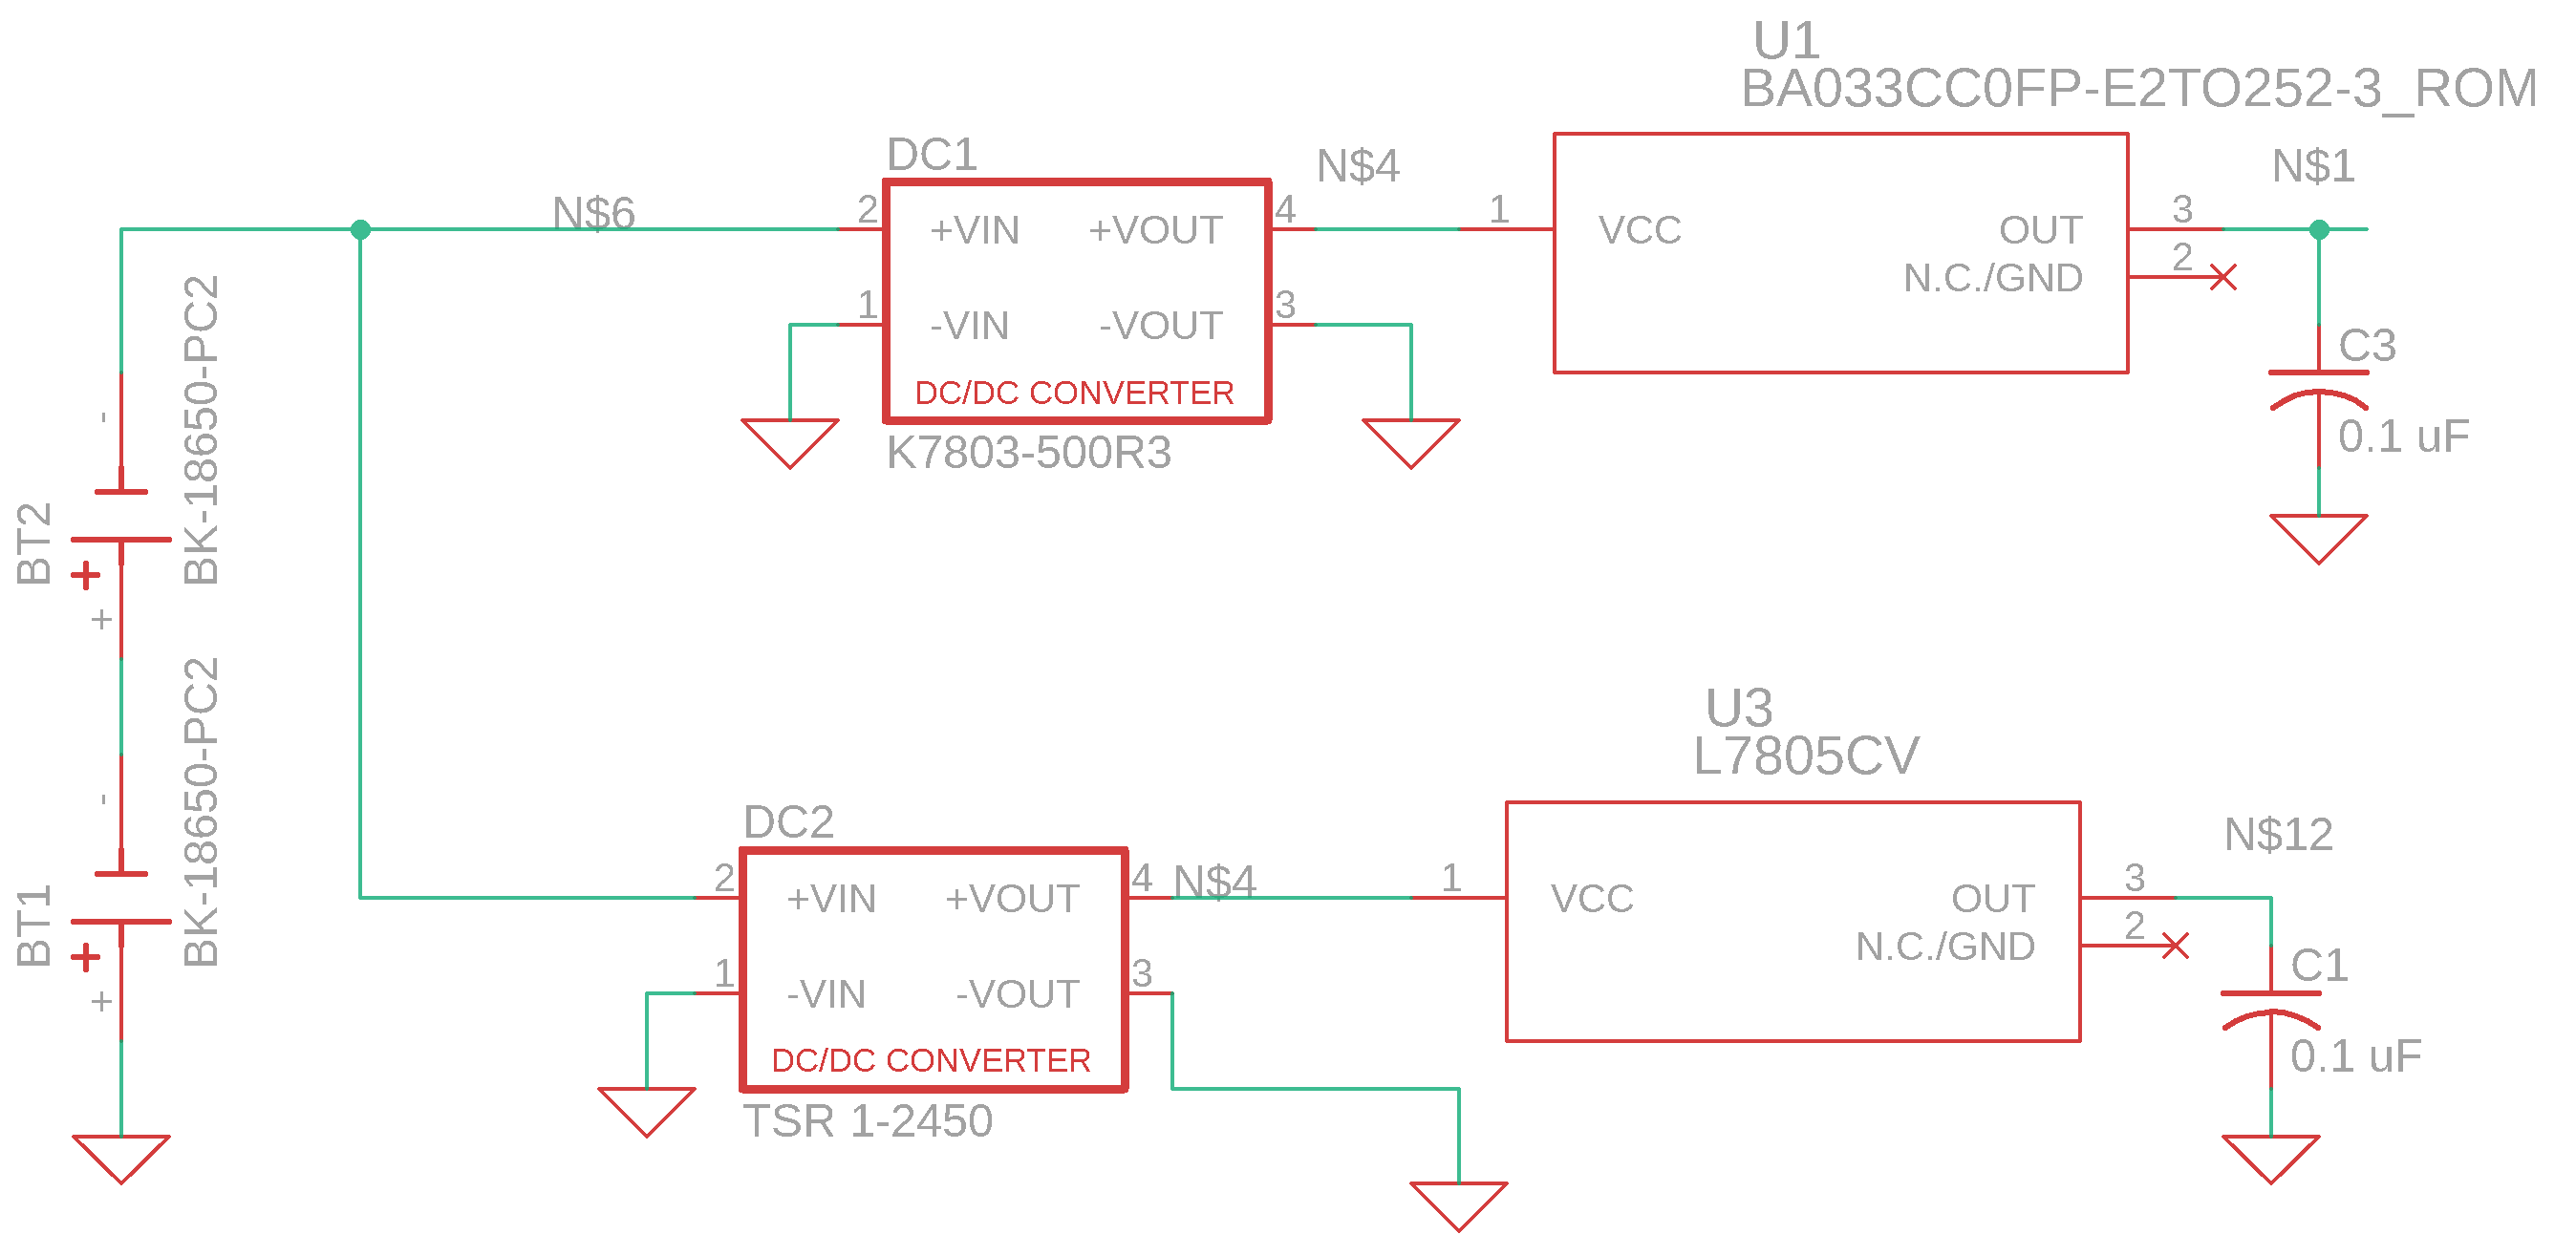
\includegraphics[width=1.6\textwidth, left]{../Modular Design/Sub-Unit-PSU/Figures/sub-unit-psu.png}
    \caption{Sub Unit PSU Schematic}
    \label{fig:sub-psu-schematic}
  \end{figure}
  \end{center}
\end{landscape}
\subsubsection{Power Analysis, Loading, Driving, and Compatibility}
The sub unit PSU operates in a very similar fashion to the main unit PSU when mains power is not available. BT1 and BT2 supply a 3.3\si{\V} (K7803-500R3) \cite{K7803500R3} and a 5\si{\V} (TSR 1-2450) \cite{TSR12450} DC/DC converter in parallel. As analyzed in the main unit PSU, both DC/DC converters require less than 6.5\si{\V} to conduct properly and since the battery is directly supplying the DC/DC converters, they will receive a nominal voltage of 7.2\si{\V} since BT1 and B2 are 3.6\si{\V} cells in series.\\ U1 (BA33BC0T) \cite{BA33BC0T} U2 (BA33BC0T) will also be compatible as analyzed above since their maximum input are above 3.3\si{\V} and 5\si{\V} respectively. As for C1 and C3, they have a voltage rating of 50\si{\V}, therefore are compatible being in parallel with the outputs of U1 and U2.
\subsubsection{Reliability \& Design Criteria}
The sub unit power supply only has to regulate the battery voltage to 3.3\si{\V} and 4\si{\V} for the MCU and Bluetooth module respectively at a high efficiency in order to achieve a 2 year life time of the design.
\subsubsection{Level of Completion}
\begin{table}[!ht]
  \begin{tabularx}{\textwidth}{|X|X|}
    \hline
    \multicolumn{2}{|X|}{Sub Unit PSU}\\
    \hline
    Integration&\begin{itemize}
                  \item 4\si{\V} Power Rail
                  \item 3.3\si{\V} Power Rail
                \end{itemize}\\
    \hline
  \end{tabularx}
\end{table}
\createfigurew{../Modular Design/Sub-Unit-PSU/Figures/sub-unit-3.3V.jpeg}{Sub unit PSU 3.3V Output Picture}{fig:sub-unit-psu-1}
\createfigurew{../Modular Design/Sub-Unit-PSU/Figures/sub-unit-4V.jpeg}{Sub unit PSU 4V Output Picture}{fig:sub-unit-psu-2}

\subsection{Main Unit}
\subsubsection{Block Diagram}
\createfigurewsvg{../Modular Design/Main-Unit/Figures/bdv5-main.svg}{Main Unit Architectural Diagram}{fig:bd-module-main-unit}
\subsubsection{State Diagram}
\begin{landscape}
\begin{figure}[!ht]
\begin{center}
  \begin{subfigure}[b]{0.6\textwidth}
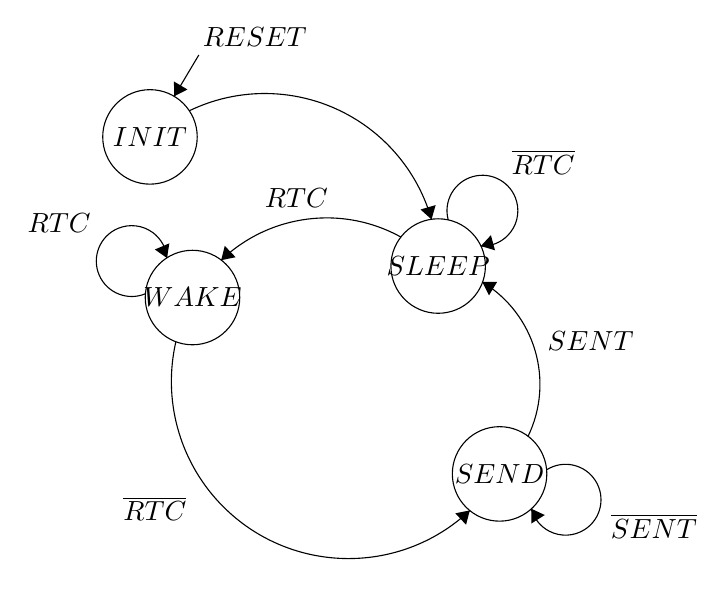
\begin{tikzpicture}[scale=0.2]
\tikzstyle{every node}+=[inner sep=0pt]
\draw [black] (36.8,-8) circle (3);
\draw (36.8,-8) node {$INIT$};
\draw [black] (55.1,-16.2) circle (3);
\draw (55.1,-16.2) node {$SLEEP$};
\draw [black] (39.5,-18.2) circle (3);
\draw (39.5,-18.2) node {$WAKE$};
\draw [black] (59,-29.4) circle (3);
\draw (59,-29.4) node {$SEND$};
\draw [black] (39.9,-2.8) -- (38.34,-5.42);
\draw (43.45,-2.3) node [above] {$RESET$};
\fill [black] (38.34,-5.42) -- (39.18,-4.99) -- (38.32,-4.48);
\draw [black] (39.29,-6.344) arc (115.82686:15.90003:11.012);
\fill [black] (54.68,-13.24) -- (54.94,-12.33) -- (53.98,-12.61);
\draw [black] (55.741,-13.281) arc (195.34019:-92.65981:2.25);
\draw (61.76,-10.43) node [above] {$\overline{RTC}$};
\fill [black] (57.81,-14.93) -- (58.71,-15.2) -- (58.45,-14.24);
\draw [black] (41.319,-15.829) arc (133.66152:60.95:9.714);
\fill [black] (41.32,-15.83) -- (42.24,-15.64) -- (41.55,-14.92);
\draw (46.1,-12.5) node [above] {$RTC$};
\draw [black] (57.903,-17.214) arc (58.79222:-25.87219:7.596);
\fill [black] (57.9,-17.21) -- (58.33,-18.06) -- (58.85,-17.2);
\draw (62.02,-20.97) node [right] {$SENT$};
\draw [black] (57.113,-31.721) arc (-46.74993:-192.99266:11.248);
\fill [black] (57.11,-31.72) -- (56.19,-31.9) -- (56.87,-32.63);
\draw (37.11,-30.8) node [below] {$\overline{RTC}$};
\draw [black] (61.977,-29.145) arc (122.62938:-165.37062:2.25);
\draw (66.04,-32.72) node [right] {$\overline{SENT}$};
\fill [black] (61.01,-31.61) -- (61.02,-32.55) -- (61.87,-32.01);
\draw [black] (36.522,-17.955) arc (293.03624:5.03624:2.25);
\draw (33.07,-13.46) node [left] {$RTC$};
\fill [black] (37.88,-15.69) -- (38.03,-14.76) -- (37.11,-15.15);
\end{tikzpicture}
\caption{Main Unit Functional State Diagram}
\label{fig:main-unit-modular-fsd-img}
  \end{subfigure}
  \begin{subfigure}[b]{0.5\textwidth}
      \begin{tabular}{c|ccc}
        STATE&\multicolumn{3}{c}{OUTPUTS}\\
        \hline
        &&&\\
        INIT&$RESET$&$\overline{RTC}$&$\overline{SENT}$\\
        SLEEP&$\overline{RESET}$&$\overline{RTC}$&$\overline{SENT}$\\
        WAKE&$\overline{RESET}$&$RTC$&$\overline{SENT}$\\
        SEND&$\overline{RESET}$&$\overline{RTC}$&$\overline{SENT}$\\
      \end{tabular}
      \caption{Main Unit Functional State Diagram: State and Outputs}
      \label{fig:main-unit-modular-fsd-state-outputs}
  \end{subfigure}
  \begin{subfigure}[b]{0.5\textwidth}
   \begin{tabular}{|c|}
    \hline
     Output List\\
    \hline
     RESET = Power on Reset\\
     SLEEP = MCU is in LPM3\\
     WAKE = RTC Timer turned on MCU\\
     SEND = Bluetooth module is sending data\\
    \hline
   \end{tabular}
      \caption{Main Unit Functional State Diagram: Output List}
      \label{fig:main-unit-modular-fsd-outputs-list}
  \end{subfigure}
\end{center}
\caption{Main Unit Functional State Diagram}
\label{fig:main-unit-modular-fsd}
\end{figure}
\end{landscape}

\subsubsection{Schematic Diagram}
\begin{landscape}
  \begin{center}
  \begin{figure}[H]
    
\includegraphics[width=\pdfpagewidth,height=0.65\textheight]{../Modular Design/Main-Unit/Figures/main-unit-and-psu.png}
    \caption{Main Unit with PSU Schematic}
    \label{fig:main-with-psu-schematic}
  \end{figure}
  \end{center}
  \end{landscape}
\subsubsection{Power Analysis}
\subsubsection{Loading, Driving, and Compatibility}
The Main Unit consists of the MSP430FR2110IPW16 MCU and the HM-10 Bluetooth module. For the MCU, it has an input voltage range from 1.8\si{\V} to 3.6\si{\V} according to it's data sheet \cite{MSP430FR2110IPW16R}. Meanwhile, the HM-10 Bluetooth module has an input voltage from 3.6\si{\V} to 6\si{\V} according to it's product listing \cite{AmazonComHiLetgo}. Due to this the MSP430FR2110 has to be supplied by the 3.3\si{V} output of the PSU and the HM-10 has to be supplied by the 5\si{\V} output of the power supply.\\
For the power available pin, according to the MSP430FR2110 data sheet, the GPIO pins can handle up to VDD =0.3\si{\V}, since in this design VDD is 3.3\si{\V} and the power available pin is at 3.3\si{\V}, it is compatible with the power sense input.\\
In order to calculate the resistor values for the green and red LEDs we used the following formula:
\begin{equation}
R = \frac{V_{cc} - V_{f}}{I_{f}}
\end{equation}
Where VCC is 3.3\si{\V} $V_{f}$ is the forward voltage for each LED and $I_{f}$ is the forward current for each LED. For the green LED \cite{GreenDiffused5mmStandard} it has a forward voltage of 2.25\si{\V} and since the MCU has a max I/O current of 2\si{\mA}, this would mean that it requires a 525\si{\ohm} resistor. Similarly, for the RED LED, it has a 2\si{\V} forward voltage and a max I/O current of 2\si{\mA}, this gives us a resistor value of  650\si{\ohm}.\\\\
Finally, for the temperature sensor (U5) \cite{TMP36GT9Z} and operational amplifier (U4) \cite{MCP6022I}, they both can be supplied by a 3.3\si{\V} supply and thus are compatible. Since the temperature sensor range for this application will be from 0\si{\celsius} to 40\si{\celsius}, at a resolution of 0.1\si{\celsius}, since there is an offset of 0.5\si{\V} by the temperature sensor gives us a range of 900 unique values so that the temperature sensor can reach its full negative temperature range. At 40\si{\celsius} the temperature sensor will be at 900\si{\milli\volt}, setting the ADC to use a 1.5\si{\V} reference. gives us a $A_{v}$ of 1.666. Setting up the op amp in a non inverting configuration, using 1\si{\kilo\ohm}, 620\si{\ohm}, 39\si{\ohm} and 5.1\si{\ohm} resistors will yield a $A_{v}$ of 1.6642.
\subsubsection{Base Times and Timing Analysis}
In order to connect both devices to each other, for communication, the best protocol to use will be UART. The MSP430FR2110 has 4 pins for UART communication using the eUSCI modules, which can detect automatically the baud-rate to be used. According to the datasheet for the HM-10 module\cite{AmazonComHiLetgo}, it can select the baud-rate to be used, which ranges from a minimum 1200 to a maximum of 230400. In the datasheet of the MSP430FR2110, the eUSCI clock frequency, UART mode, can reach a maximum of 5MHz, which means it can reach the maximum baud-rate of the Bluetooth module and can also select lower baud-rates, according to the formula:
\begin{equation}
	Clk Frequency = Baudrate \cdot 16
	\label{eq:UART Frequency}
\end{equation}
This means if we select the maximum baud-rate of the HM-10 module, which is 230400, using the formula, we would need a frequency of 3.68MHz, which is still below the maximum frequency the eUSCI module on the MSP430FR2110. This will allow us to be able to use the HM-10 communicate via UART with the MSP430FR2110.\\
\subsubsection{Software Support}
\createfigurel{../Modular Design/Main-Unit/Figures/main-unit-main-function.png}{Main Unit Main Function}{fig:main-unit-main-function}
\createfigurel{../Modular Design/Main-Unit/Figures/main-unit-rtc-isr.png}{Main Unit RTC ISR}{fig:main-unit-rtc-isr}
\createfigurel{../Modular Design/Main-Unit/Figures/main-unit-bluetooth-isr.png}{Main Unit Bluetooth ISR}{fig:main-unit-bluetooth-isr}
\subsubsection{Memory Requirements}
The program itself consists of 300 instructions, which assuming a 1 to 10 conversion ration between C and Assembly language yields a total of 3000 bytes of program data. Since the main unit's source code has two buffers for RX and TX of 83 bytes each plus the buffer for lot number (30 bytes), the string versions of the error enums (56 bytes), the error enum (1 byte) and the error state (1 byte) gives us a size of 344 bytes of data memory.
\subsubsection{Reliability \& Design Criteria}
The main unit was the backbone of the whole system, without
\subsubsection{Level of Completion}

\subsection{Sub Unit}
\subsubsection{Block Diagram}
\subsubsection{State Diagram}
\subsubsection{Schematic Diagram}
\subsubsection{Power Analysis}
\subsubsection{Loading, Driving, and Compatibility}
\subsubsection{Base Times and Timing Analysis}
\subsubsection{Software Support}
\subsubsection{Memory Requirements}
\subsubsection{Reliability \& Design Criteria}
\subsubsection{Level of Completion}


\section{System Integration}
\subsection{System Integration Plan}
\begin{enumerate}
  \item Connect both MSP430FR2311 to the 3.3\si{\V} supply with their respective power supplies.
  \item Connect the LEDs with their respective resistors with the MCU pins and ground.
        \begin{itemize}
         \item To verify that the MSP430FR2311s are working, an LED will be lit by a push button in order by the MCU.
        \end{itemize}
  \item Connect the power sense pin to a GPIO of the main unit.
        \begin{itemize}
         \item  To verify that this is working, an LED shall be lit by the MCU when power is absent and off when power is present.
        \end{itemize}
  \item Connect the HM-10 bluetooth modules to the 5\si{\V} supply of their respective power supplies.
  \item Connect the UART pins from the MCU to the HM-10s.
        \begin{itemize}
         \item To verify this, we shall check if it can send a ``Hello World'' to a serial monitor.
        \end{itemize}
  \item Connect the external temperature sensor to the 3.3\si{\V} supply and connect the output pin to a ADC pin on the MCU.
        \begin{itemize}
         \item In order to verify that this is working, we shall use the debugger to see the ADC registers.
        \end{itemize}
\end{enumerate}
\subsection{Host/Multi-unit Software Support}
The software that binds main unit and the host computer is a BASH script. This script connects the main unit to the host computer via bluetooth and redirects the serial monitor of the main unit transmitter to standard output and to a log-file that is written to home folder of the current user.
\subsection{System reliability \& Design Criteria}
As mentioned previously, the reliability of the main and sub units is paramount to ensure that the insulin vials are safe to use. The reliability of the host computer was also essential because it serves as the log file creator for the entire system. A major design consideration for this design was for the client to be able to integrate this product within their existing assembly process for insulin and be relatively inexpensive for repair and replace both the main ans sub units. For the log-file creator, BASH was chosen since it is a battle tested shell for Linux operating systems that themselves are reliable and battle tested.
\begin{landscape}
\subsection{Level of Completion}
  \begin{table}[!ht]
    \begin{tabularx}{\textwidth}{|X|X|}
      \hline
      \multicolumn{2}{|X|}{Main Unit}\\
      \hline
      Integration&\begin{itemize}
                    \item Battery Backup Mains Power Supply
                    \item Main Unit
                  \end{itemize}\\
                  \hline
      Functionality&\begin{itemize}
          \item ADC 12 Initialization using VEREF+ and VEREF- reference and input channel 7.
          \item UART initialization at 9600 baud with receiver interrupts enabled.
          \item Forwards errors from sub units along with the current time.
          \item Verifies the availability of mains power and forwards that information to the host computer.
        \end{itemize}\\
      \hline
    \end{tabularx}
    \caption{Main Unit Level of Completion Table}
    \label{tab:main-unit-completion-table}
  \end{table}
  \begin{table}[!ht]
    \begin{tabularx}{\textwidth}{|X|X|}
      \hline
      \multicolumn{2}{|X|}{Main Unit}\\
      \hline
      Integration&\begin{itemize}
                    \item Power Supply
                    \item Main Unit
                  \end{itemize}\\
                  \hline
      Functionality&\begin{itemize}
          \item ADC 12 Initialization using VEREF+ and VEREF- reference and input channel 7.
          \item UART initialization at 9600 baud with receiver interrupts enabled.
          \item RTC initialization at once twice per day.
          \item RTC runs the ADC 100 times and averages the results and checks if the temperature meets compliance.
          \item If an error is raised, the UART is activated and sends an error along with the lot number.
        \end{itemize}\\
      \hline
    \end{tabularx}
    \caption{Sub Unit Level of Completion Table}
    \label{tab:sub-unit-completion-table}
  \end{table}
\end{landscape}
\createfigurew{../System Integration/Figures/log-file-picture.jpeg}{Log File Demo}{fig:log-file-demo}
Here is the \href{https://youtu.be/BvUFnom23P8}{link} for the demo of the log file.

\subsection{User’s Guide}
\subsubsection{Installation}
\large{Main Unit}
\normalsize
\linespread{2.0}
\begin{enumerate}
  \item Charge the 18650 batteries for the main unit.
  \item Place the batteries in the holder with the positive terminals facing up.
  \item Place main unit in an area that will be the center of where the sub units will be stored in.
  \item Connect the main unit to mains power.
\end{enumerate}
\large{Sub Unit}
\normalsize
\linespread{2.0}
\begin{enumerate}
  \item Charge the 18650 batteries for the sub unit.
  \item Program the individual sub unit with a LOT number.
  \item Place the batteries in the holder with the positive terminals facing up.
  \item Glue the sub unit to the insulin box.
\end{enumerate}
\subsubsection{Setup}
\large{Main Unit}
\normalsize
\begin{enumerate}
  \item Download \href{https://pypi.org/project/ble-serial/}{ble-serial} or any other BLE serial monitor and follow the connection instructions to connect the main unit.
  \item run log-file.bash passing the virtual serial port as an argument.
  \item Verify that the log file is being created in the home folder of the current user.
\end{enumerate}
\large{Sub Unit\\}
\normalsize
No setup is required.
\subsubsection{Operation}
The log file that is in the user's home folder on the host computer will contain the log data in the following format: date (year, month, day, hour:minute:second), power status and all error codes for any sub units.
\large{Operating Conditions}
\normalsize
\begin{itemize}
  \item Temperature: -20\si{\C} to 95\si{\C}
  \item Main unit mains input voltage: 85\si{\V} to 264\si{\V}.
  \item Sub Unit Battery Life: 2 years.
  \item Main Unit Battery life: 30 days.
\end{itemize}

\section{Closing Section}
\subsection{Conclusion}
In summary, we were successfully able to create a design that ensures that ensures the safe storage of insulin. The Insulin Temperature Warning System's design was split up into a main unit, a sub unit and a host computer that runs the log file software. The sub units verify that the insulin meets temperature safety compliance and if not sends a error to the main unit. The main unit monitors the presence of mains power along with forwarding the current date, power status and any errors from the sub units. The host computer receives the messages from the main unit logs them into a log file.
\subsection{Future Work}
The next step for furthering the Insulin Temperature Warning System is to create a PCB version with surface mount components in order to both decrease size and cost. Furthermore, adapting the software to accept more medications or even create a version that can be programmed by a non-engineer for a new medication's storage guidelines could be within the realm of possibility.
\subsection{Reflections/Recommendations}
On retrospection, this design can be streamlined by compressing the roles of the main and sub units into a single design that leverages software for the connection of the Bluetooth module. Furthermore, we believe that using micro-controllers with open source designs and software will help greatly in the speed of prototyping and the fixing of bugs in both the design and software.

\bibliographystyle{IEEEtranN}
\bibliography{../References/references.bib}

\end{document} 
